\section{Auswertung}
\label{sec:Auswertung}

\subsection{Invertierter Linearverstärker}
\label{sec:Invertierter_Linearverstärker}
Die Spannung des Ausgangssignals $U_2$ wird in Abhängigkeit von der verwendeten Frequenz~$f$ gemessen. Mithilfe
der bekannten Widerstände $R_1$ und $R_2$ sowie Formel~\eqref{eq:invert} werden die theoretischen Verstärkungen für die drei eingebauten
Widerstandskombinationen ausgerechnet. Es ergibt sich
\begin{align*}
  V_{1, \mathrm{theo}} &= \frac{\qty{100}{\kilo\ohm}}{\qty{1}{\kilo\ohm}} = \num{100} \\
  V_{2, \mathrm{theo}} &= \frac{\qty{150}{\kilo\ohm}}{\qty{10}{\kilo\ohm}} = \num{15} \\
  V_{3, \mathrm{theo}} &= \frac{\qty{68}{\kilo\ohm}}{\qty{330}{\ohm}} \approx \num{179}. \\  
\end{align*}

Wird die tatsächlich gemessenen Verstärkung $V$ in Abhängigkeit von der Frequenz $f$ in einem doppelt-logarithmischen Diagramm dargestellt,
ergeben sich Graphen, die zunächst annähernd konstant verlaufen und ab einem bestimmten Punkt linear abfallen. Die entsprechenden Plots
der experiementellen Daten sind in \autoref{fig:plots_inv} dargestellt.

\begin{figure}
  \begin{subfigure}[c]{0.9\textwidth}
    \centering
    \includegraphics[height=6.4cm]{build/invert1.pdf}
    \caption{$V_{1, \mathrm{theo}} = 100$}
  \end{subfigure}
  \begin{subfigure}[c]{0.9\textwidth}
    \centering
    \includegraphics[height=6.4cm]{build/invert2.pdf}
    \caption{$V_{2, \mathrm{theo}} = 15$}
  \end{subfigure}
  \begin{subfigure}[c]{0.9\textwidth}
    \centering
    \includegraphics[height=6.4cm]{build/invert3.pdf}
    \caption{$V_{3, \mathrm{theo}} = 179$}
  \end{subfigure}
  \caption{Doppellogarithmische Plots der bei verschiedenen Freqeunzen $f$ zu beobachtenden Verstärkungen $V$.}
  \label{fig:plots_inv}
\end{figure}

Die gemittelte Leerlaufverstärkung $V$ ergibt sich jeweils als Mittelwert der in \autoref{fig:plots_inv} als konstant zu betrachtenden
Messwerte. Es folgt
\begin{align*}
  V_1 &= \num{92+-5} \\
  V_2 &= \num{15.1+-0.4} \\
  V_3 &= \num{129+-11}. \\
\end{align*}

Die Grenzfrequenz $f_{\mathrm{Grenz}}$ des Schaltkreises wird als die Frequenz definiert, bei der die Verstärkung $V$ den 
Wert $\frac{V_{\symup{i}}}{\sqrt{2}}$ annimmt. Zur Berechnung dieser Grenzfrequenzen werden mithilfe der \texttt{python}-Erweiterung
\texttt{scipy}~\cite{scipy} lineare Fits der Messwerte von den Flanken in \autoref{fig:plots_inv} erstellt. Durch einfaches Gleichsetzen
der sich ergebenden Fitfunktion mit $\ln\left(\frac{V_{\symup{i}}}{\sqrt{2}}\right)$ und Umformen ergeben sich die 
Grenzfrequenzen~$f_{\mathrm{Grenz}}$. Diese, sowie die Fitparameter der drei verschiedenen Verstärkungen sind in \autoref{tab:inv_f_Grenz}
dargestellt.

\begin{table}
  \centering
  \caption{Leerlaufverstärkung, Fitparameter der Flankenfits aus \autoref{fig:plots_inv} und daraus resultierende Grenzfrequenzen $f_{\mathrm{Grenz}}$, sowie das Bandbreitenprodukt.}
  \label{tab:inv_f_Grenz}
  \begin{tabular}{S S S S S S}
    \toprule
    {$V_{\mathrm{theo}}$} & {$V_{\mathrm{i}}$} & {$m$} & {$b$} & {$f \mathbin{/} \unit{\kilo\hertz}$} & {$V_{\symup{i}} \cdot f_{\mathrm{Grenz}} \mathbin{/} \unit{\kilo\hertz}$} \\
    \midrule
    100 & \num{92+-5} & \num{-0.931+-0.023} & \num{6.37+-0.09} & \num{10.5+-1.3} & \num{9.7(1.1)e2} \\
     15 & \num{15.1+-0.4} & \num{-0.617+-0.026} & \num{4.86+-0.11} & \num{57+-14} & \num{5.3(1.4)e3} \\
    179 & \num{129+-11} & \num{-0.881+-0.024} & \num{6.21+-0.09} & \num{6.9+-1.0} & \num{6.3(1.0)e2} \\
    \bottomrule
  \end{tabular}
\end{table}

Neben den Leerlaufverstärkungungen und den Grenzfrequenzen wird auch die Phasenverschiebung zwischen Eingangs- und Ausgangsspannung betrachtet.
Diese ist ebenfalls Freqeunzabhängig und wird in \autoref{fig:invert_phase} dargestellt.

\begin{figure}
  \centering
  \includegraphics{build/invert_phase.pdf}
  \caption{Messwerte der Phasenverschiebung $\varphi$ zwischen der Eingangsspannung~$U_1$ und Ausgangsspannung $U_2$ für 
  die verschiedenen Widerstandskombinationen.}
  \label{fig:invert_phase}
\end{figure}


\subsection{Integrator}
Für die Schaltung eines Integrators ergibt sich mit den Werten des Kondensators $R_1=\qty{10}{\kilo\ohm}$ und des Kondensators $C=\qty{100}{\nano\farad}$ für die Zeitkonstante
\begin{equation*}
  \tau_{\mathrm{int, theo}} = RC = \qty{1}{\milli\second}.
\end{equation*}
Ein experimenteller Wert für die Zeitkonstante lässt sich bestimmen, indem erneut in einem doppellogarithmischen Diagramm die Verstärkung gegen die Frequenz aufgetragen wird. Erneut wird 
mithilfe der \texttt{python}-Erweiterung \texttt{scipy}~\cite{scipy} ein linearer Fit der Messwerte durchgeführt. In \autoref{fig:integrator_exp} ist das doppellogarithmische Diagramm mit 
eingezeichneter Fitfunktion zu sehen.

\begin{figure}
  \centering
  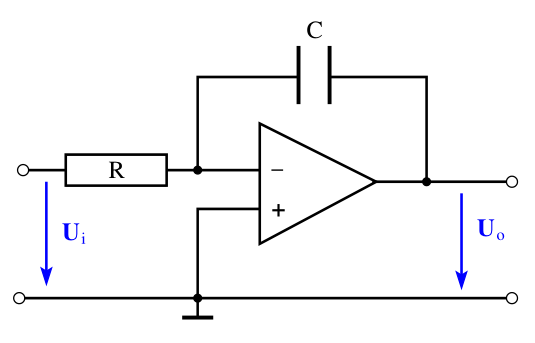
\includegraphics{build/integrator.pdf}
  \caption{Doppellogarithmischer Plot der Messwerte der Verstärkung von der Integratorschaltung abhängig von der Frequenz mit eingezeichneter Fit- und Theoriefunktion.}
  \label{fig:integrator_exp}
\end{figure}

Die Fitfunktion liefert die logarithmische Verstärkung abhängig von der logarithmischen Frequenz gemäß
\begin{equation*}
  \ln(V) = m \ln\left(\frac{f}{\unit{\hertz}}\right) + b.
\end{equation*}
Durch Exponenzieren und Umformen wird 
\begin{equation*}
  V = f^{m}\symup{e}^{b}
\end{equation*}
erreicht. Durch einen Koeffizientenvergleich mit \autoref{eq:integrator2} folgt, dass
\begin{align*}
  m &\approx -1 & e^{b} &=\frac{1}{RC} \\
\end{align*}
gelten muss. Die Fitparameter ergeben sich zu
\begin{align*}
  m &= \num{-0.930+-0.008} & b&= \num{5.052+-0.033},
\end{align*}
woraus für die Zeitkonstante
\begin{equation*}
  \tau_{\mathrm{int, exp}} = \qty{6.40+-0.21}{\milli\second}
\end{equation*}
folgt.

Nach \autoref{eq:integrator1} wirkt diese Schaltung als Integrator. Dies lässt sich experiementell überprüfen, indem verschiedene Wechselspannungen als Eingangssignal verwendet werden
und die Ausgangsspannung damit verglichen wird. In \autoref{fig:scope_int} ist der Bildschirm des Oszilloskops bei drei verschiedenen Wechselspannungen zu sehen. Es ist für alle Eingangssignale
zu beobachten, dass diese integriert werden.

\begin{figure}
  \begin{subfigure}[c]{0.9\textwidth}
    \centering
    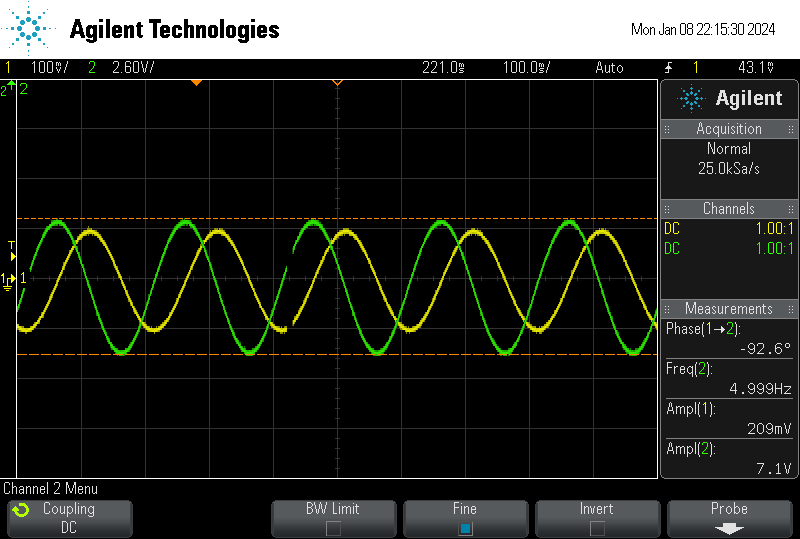
\includegraphics[height=6.4cm]{content/scope/scope_1.png}
    \caption{Sinusspannung, $f=\qty{5}{\hertz}$}
  \end{subfigure}
  \begin{subfigure}[c]{0.9\textwidth}
    \centering
    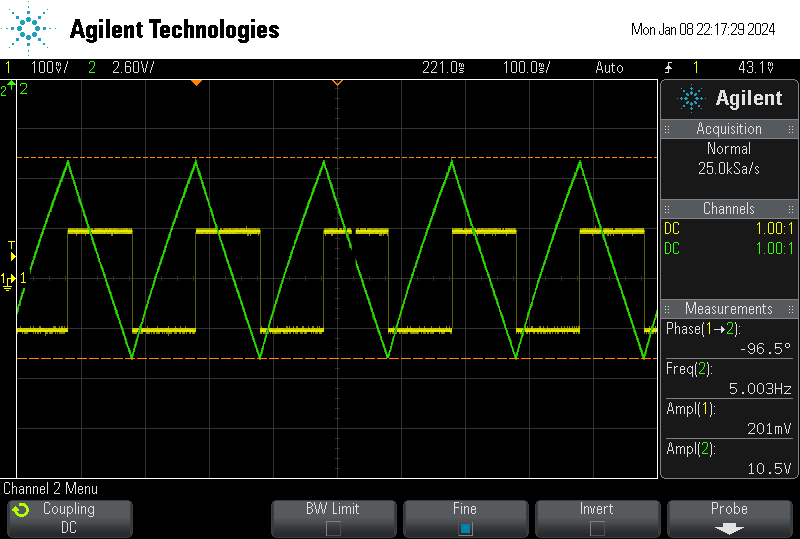
\includegraphics[height=6.4cm]{content/scope/scope_4.png}
    \caption{Rechteckspannung, $f=\qty{5}{\hertz}$}
  \end{subfigure}
  \begin{subfigure}[c]{0.9\textwidth}
    \centering
    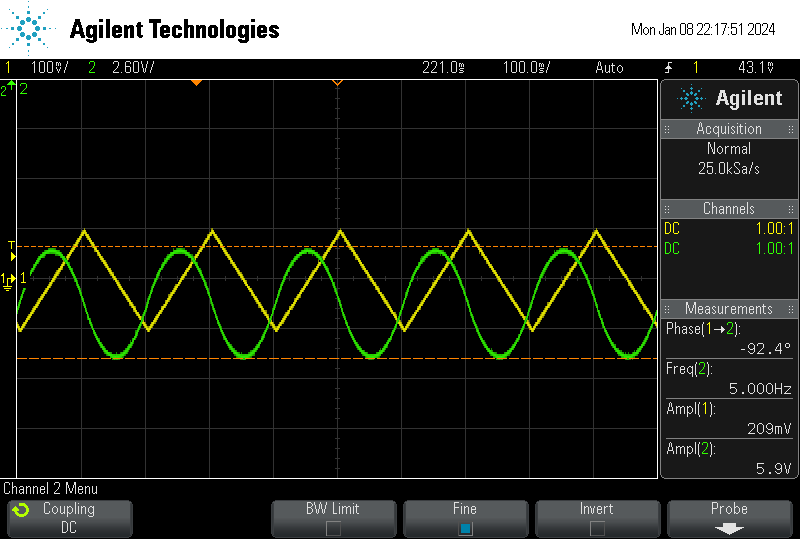
\includegraphics[height=6.4cm]{content/scope/scope_5.png}
    \caption{Dreieckspannung, $f=\qty{5}{\hertz}$}
  \end{subfigure}
  \caption{Bilder des Oszilloskopschirms bei verschiedenen angelegten Wechselspannungen für die Integratorschaltung.}
  \label{fig:scope_int}
\end{figure}

\subsection{Differenzierer}
Für den Differenzierer wird analog zum Integrator vorgegangen, die Zeitkonstante wird mit $R_2=\qty{100}{\kilo\ohm}$ und $C=\qty{22}{\nano\farad}$ zu 
\begin{equation*}
  \tau_{\mathrm{diff, theo}} = RC = \qty{2,20}{\milli\second}
\end{equation*}
berechnet. Der Koeffizientenvergleich erfolgt mit \autoref{eq:differenzierer2}. Demnach muss
\begin{align*}
  m &\approx 1 & e^{b} &={RC} \\
\end{align*}
gelten. In \autoref{fig:differenzierer_exp} ist der entsprechende Plot dargestellt.
\begin{figure}
  \centering
  \includegraphics{build/differentiator.pdf}
  \caption{Doppellogarithmischer Plot der Messwerte der Verstärkung von der Differenzierschaltung abhängig von der Frequenz mit eingezeichneter Fit- und Theoriefunktion.}
  \label{fig:differenzierer_exp}
\end{figure}
Die Parameter des Fits lauten
\begin{align*}
  m &= \num{-1.0159+-0.0027} && \text{und}& b&= \num{6.658+-0.010}.
\end{align*}
Auf den ersten Blick wird klar, dass diese Werte nicht mit der Theorie vereinbar sind. Gründe für die große Diskrepanz werden in \autoref{sec:Diskussion} erörtert. Aufgrund der
großen Abweichung von der Theorie wird auf eine weitere Berechnung der Zeitkonstanten verzichtet.

Werden hier erneut drei verschiedene Wechselspannungen als Eingangssignal verwendet, lässt sich nicht die nach \autoref{eq:differenzierer1} zu erwartende ableitende Wirkung des 
Differenzierers beobachten. Stattdessen wird in \autoref{fig:scope_diff} deutlich, dass hier, wie zuvor, integriert wird.

\begin{figure}
  \begin{subfigure}[c]{0.9\textwidth}
    \centering
    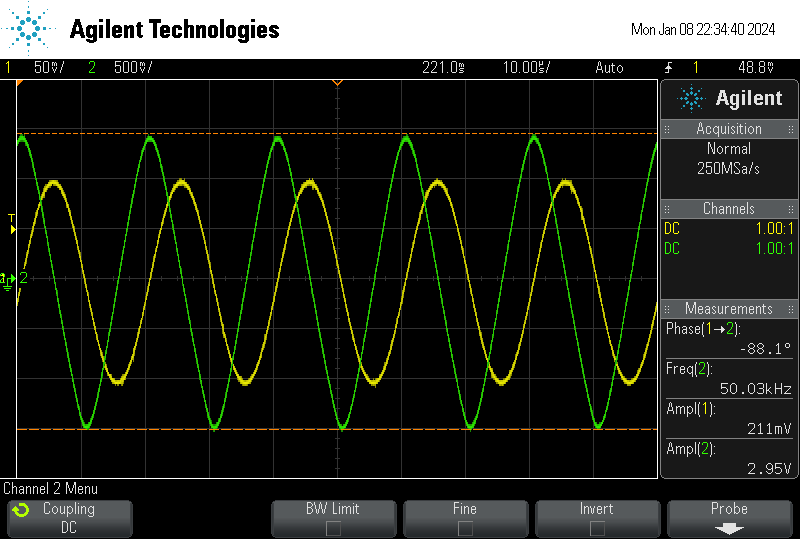
\includegraphics[height=6.4cm]{content/scope/scope_8.png}
    \caption{Sinusspannung, $f=\qty{50}{\kilo\hertz}$}
  \end{subfigure}
  \begin{subfigure}[c]{0.9\textwidth}
    \centering
    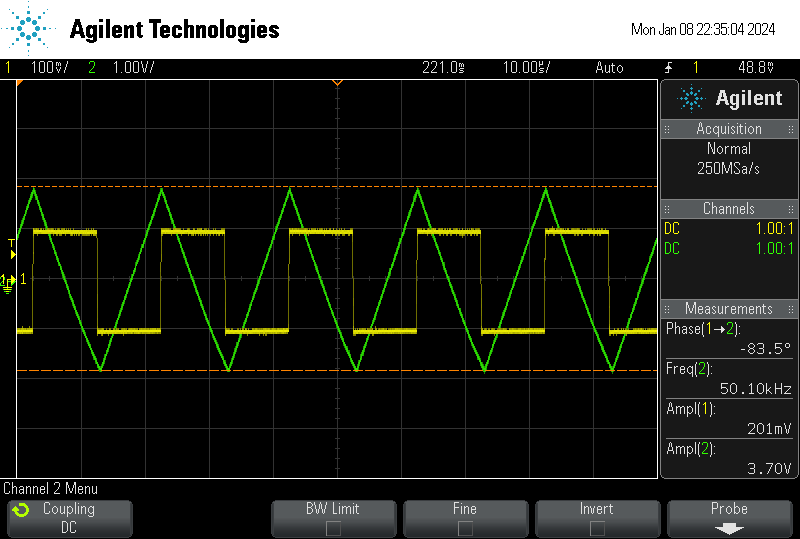
\includegraphics[height=6.4cm]{content/scope/scope_9.png}
    \caption{Rechteckspannung, $f=\qty{50}{\kilo\hertz}$}
  \end{subfigure}
  \begin{subfigure}[c]{0.9\textwidth}
    \centering
    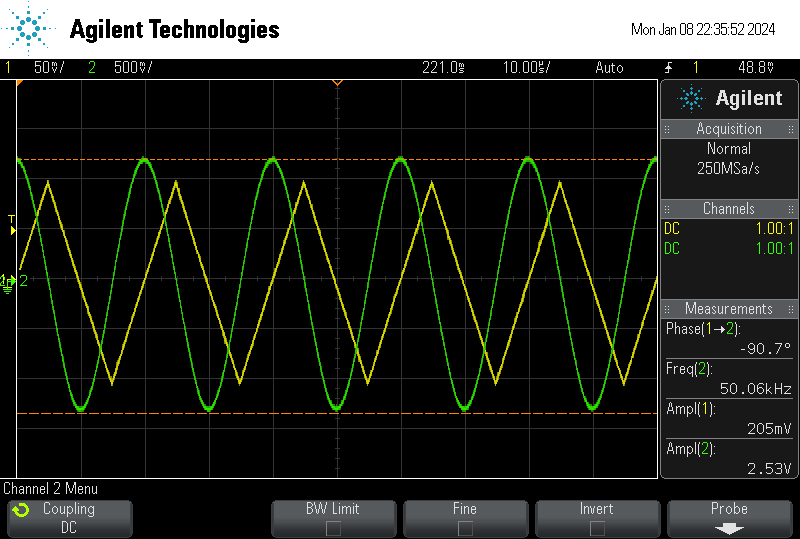
\includegraphics[height=6.4cm]{content/scope/scope_12.png}
    \caption{Dreieckspannung, $f=\qty{50}{\kilo\hertz}$}
  \end{subfigure}
  \caption{Bilder des Oszilloskopschirms bei verschiedenen angelegten Wechselspannungen für die Differentiatorschaltung.}
  \label{fig:scope_diff}
\end{figure}

\subsection{Schmitt-Trigger}
Mithilfe von \autoref{eq:schmitt_trigger} wird die für die verwendeten Widerstände $R_1=\qty{10}{\kilo\ohm}$ und $R_2=\qty{100}{\kilo\ohm}$ theoretische Schwellenspannung 
\begin{equation*}
  U_{\mathrm{kipp, theo}} = \pm \frac{R_1}{R_2} U_{\symup{B}} = \pm \frac{\qty{10}{\kilo\ohm}}{\qty{100}{\kilo\ohm}} \qty{15}{\volt} = \pm\qty{1,5}{\volt}
\end{equation*}
berechnet.
Durch langsames Erhöhen der Eingangsspannung bis zum Kipppunkt wird die experiementelle Schwellenspannung 
\begin{equation*}
  U_{\mathrm{kipp, exp}} = \qty{1,503}{\volt}
\end{equation*}
bestimmt. In \autoref{fig:scope_schmitt} ist der Oszilloskopschirm knapp überhalb der Schwellenspannung zu sehen.
\begin{figure}
  \centering
  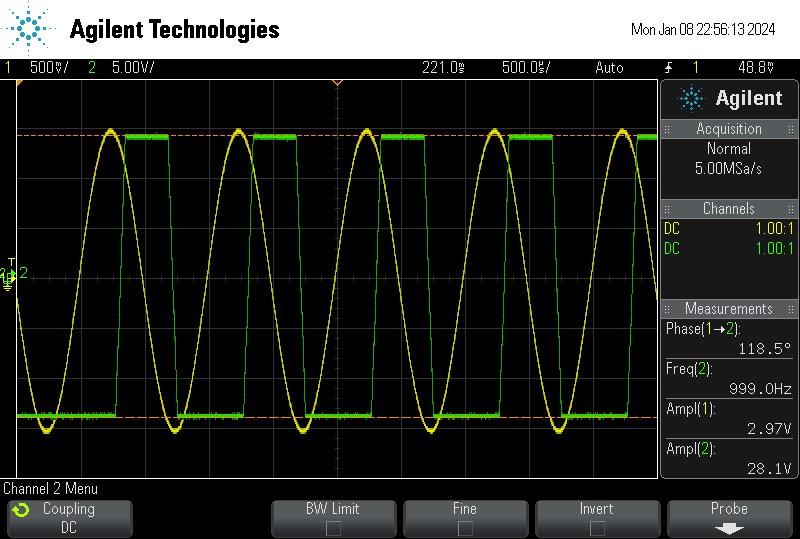
\includegraphics[height=6.4cm]{content/scope/scope_15.png}
  \caption{Bild des Oszilloskopschirms des Schmitt-Triggers bei einer Eingangsspannung von $U=\qty{1,503}{\volt}$.}
  \label{fig:scope_schmitt}
\end{figure} 

\subsection{Generator}
Für den Generator werden die Widerstände $R_1=\qty{10}{\kilo\ohm}$, $R_20=\qty{10}{\kilo\ohm}$, $R_3=\qty{1}{\kilo\ohm}$, sowie ein Kondensator mit $C=\qty{1}{\micro\farad}$ verwendet.
Mit den Formeln \eqref{eq:freq_generator} und \eqref{eq:amplitude_generator} für die Frequenz und Amplitude werden diese zu
\begin{align*}
  \nu_\text{a} &= \frac{R_2}{4C R_1 R_3} =\qty{2,5}{\kilo\hertz} \\
  U_0 &= U_\text{max} \frac{R_1}{R_2} =\qty{1,5}{\volt} \\
\end{align*}
berechnet. Experimentelle Werte dafür lassen sich aus \autoref{fig:scope_generator1} bestimmen.
\begin{figure}
  \centering
  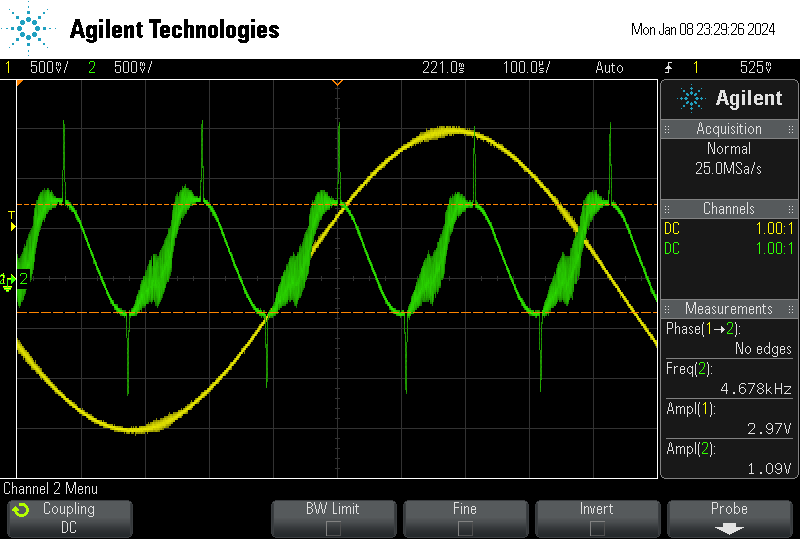
\includegraphics[height=6.4cm]{content/scope/scope_16.png}
  \caption{Bild des Oszilloskopschirms für die Generatorschaltung.}
  \label{fig:scope_generator1}
\end{figure}
Es ergibt sich
\begin{align*}
  \nu_{\mathrm{a, exp}} &= \qty{4,678}{\kilo\hertz} \\
  U_{0, \mathrm{exp}} &= \qty{1,09}{\volt}.
\end{align*}

Für die weitergehende Generatorschaltung mit variierender Amplitude wird die Schaltung gemäß des Schaltplans
\autoref{fig:generator2} umgebaut. Als Kapazität des Kondensators wird $C=\qty{100}{\nano\farad}$ gewählt, sodass sich mit der
Widerstandskonstanten $R=\qty{10}{\kilo\ohm}$ und \autoref{eq:T} eine theoretische Periodendauer von
\begin{equation*}
  T_{\mathrm{theo}} = \qty{6,28}{\milli\second}
\end{equation*}
ergibt. Zur experiementellen Bestimmung der Periodendauer wird mithilfe des Oszilloskops die abklingende Schwingung sichtbar gemacht.
Dies ist in \autoref{fig:scope_generator2} zu sehen, wobei zu beachten ist, dass aus, in \autoref{sec:Diskussion} näher diskutierten, möglichen 
Gründen die eingekoppelte Rechteckspannung nicht zeitgleich mit der gedämpften Schwingung sichtbar ist.
\begin{figure}
  \begin{subfigure}[c]{0.49\textwidth}
    \centering
    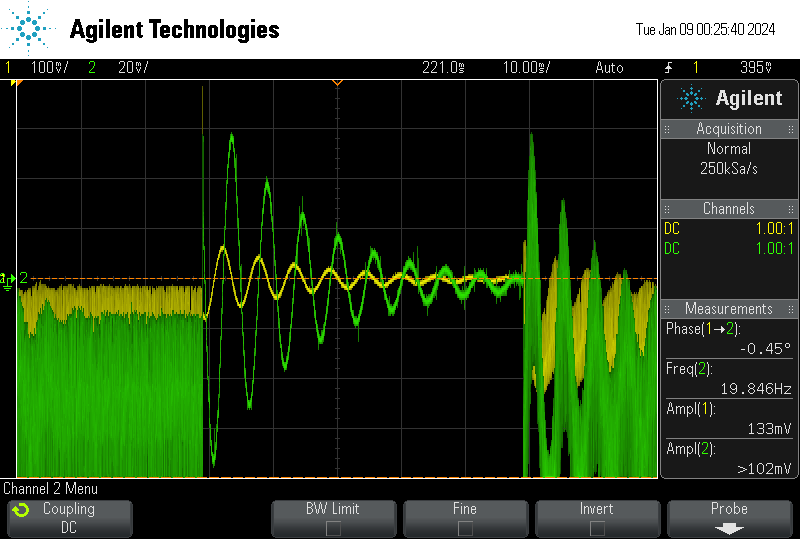
\includegraphics[width=\textwidth]{content/scope/scope_19.png}
    \caption{Gedämpfte Schwingung für $f=\qty{10}{\hertz}$. Die Rechteckspannung ist nicht zu erkennen.}
    \label{fig:scope_generator2_a}
  \end{subfigure}
  \begin{subfigure}[c]{0.49\textwidth}
    \centering
    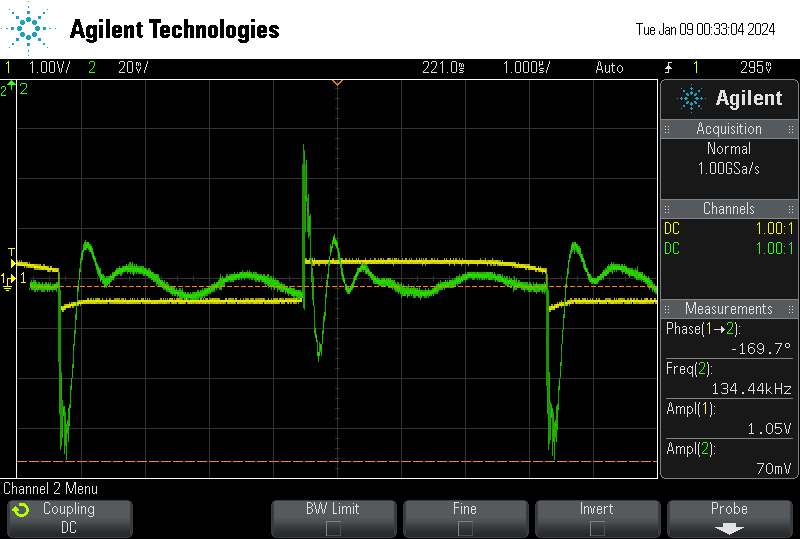
\includegraphics[width=\textwidth]{content/scope/scope_20.png}
    \caption{Kaum sichtbare gedämfte Schwingung bei sichtbarer Rechteckspannung mit $f=\qty{131}{\kilo\hertz}$.}
  \end{subfigure}
  \caption{Oszilloskopschirm der Generatorschaltung mit variierender Amplitude für verschiedene Frequenzen.}
  \label{fig:scope_generator2}
\end{figure}
\begin{figure}
  \begin{subfigure}[c]{0.49\textwidth}
    \centering
    \includegraphics[width=\textwidth]{build/generator_scope.pdf}
  \end{subfigure}
  \begin{subfigure}[c]{0.49\textwidth}
    \centering
    \includegraphics[width=\textwidth]{build/generator_scope_zoomed.pdf}
  \end{subfigure}
  \caption{Plot des Oszilloskopschirms aus \autoref{fig:scope_generator2_a}. Rechts: Zoom der relevanten Schwingung im Signal mit eingezeichneten
  lokalen Maxima.}
  \label{fig:plot_generator}
\end{figure}
Zur Bestimmung der Periodendauer der Schwingung werden die Daten aus \autoref{fig:scope_generator2_a} in \autoref{fig:plot_generator} geplottet
und die lokalen Extrema werden bestimmt. Aus dem mittleren Abstand dieser wird die experiementelle Periodendauer zu
\begin{equation*}
  T_{\mathrm{exp}} = \qty{5.56+-0.32}{\milli\second}
\end{equation*}
bestimmt.